% Figura 3 — pipeline de entrega: do CI verde ao smoke pela borda.
\documentclass[11pt,tikz,border=6pt]{standalone}
\usepackage{fontspec}
\setmainfont{LibertinusSerif}[Extension=.otf, UprightFont=*-Regular,
  BoldFont=*-Bold, ItalicFont=*-Italic, BoldItalicFont=*-BoldItalic, Ligatures=TeX]
\setmonofont{Inconsolatazi4-Regular}[Extension=.otf, BoldFont=Inconsolatazi4-Bold,
  Ligatures=TeX, Scale=0.92]
\usetikzlibrary{arrows.meta,calc,fit,shapes.geometric}

\definecolor{tinta}{HTML}{1F2933}
\definecolor{petroleo}{HTML}{0F766E}
\definecolor{ambar}{HTML}{B45309}
\definecolor{fundo}{HTML}{F5F7F8}

\begin{document}
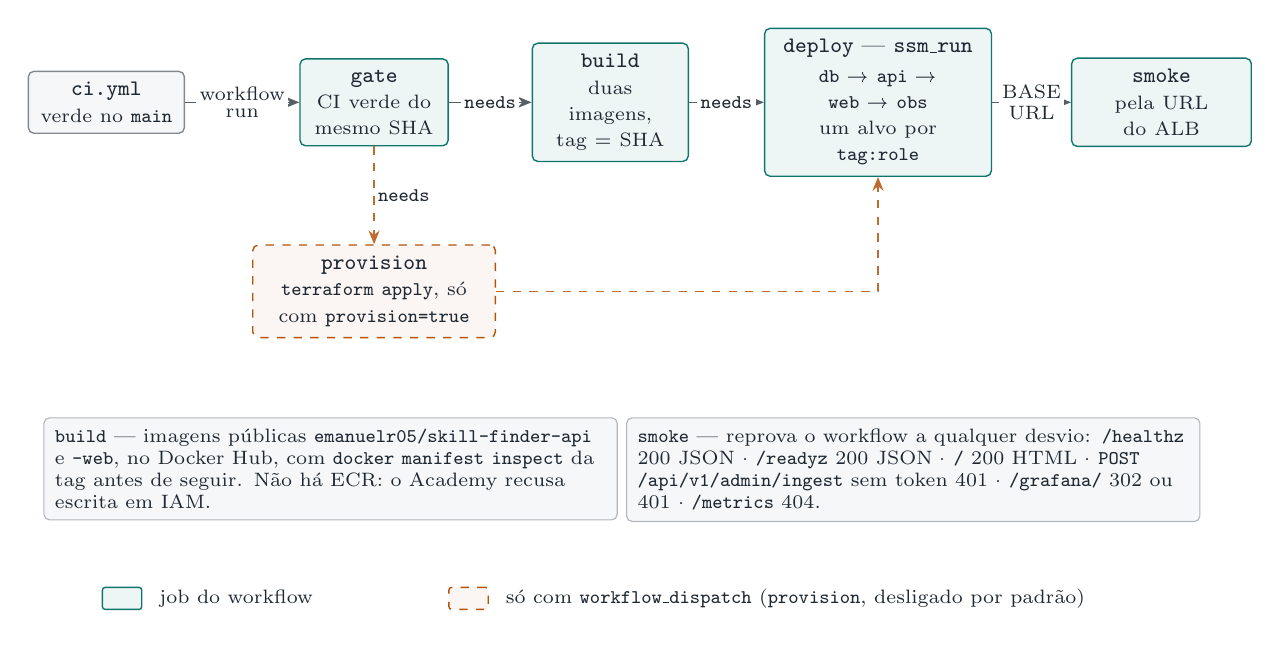
\begin{tikzpicture}[
    font=\footnotesize,
    >={Stealth[length=5pt,width=4pt]},
    etapa/.style={draw=petroleo, line width=0.5pt, fill=petroleo!7, rounded corners=2pt,
      align=center, inner sep=4pt, text=tinta},
    externo/.style={draw=tinta!55, line width=0.5pt, fill=fundo, rounded corners=2pt,
      align=center, inner sep=4pt, text=tinta},
    manual/.style={draw=ambar, dashed, line width=0.5pt, fill=ambar!5, rounded corners=2pt,
      align=center, inner sep=4pt, text=tinta},
    nota/.style={draw=tinta!35, line width=0.4pt, fill=fundo, rounded corners=2pt,
      align=left, inner sep=4pt, text=tinta, font=\scriptsize},
    seta/.style={->, line width=0.5pt, draw=tinta!75},
    ctrl/.style={->, dashed, line width=0.5pt, draw=ambar!85},
    rot/.style={font=\scriptsize, text=tinta, fill=white, inner sep=1.2pt, inner ysep=0.5pt},
  ]

  % ---------- a cadeia principal ----------
  \node[externo, text width=1.7cm] (ci) at (1.0,7.6)
    {\texttt{ci.yml}\\{\scriptsize verde no \texttt{main}}};
  \node[etapa, text width=1.6cm] (gate) at (4.4,7.6)
    {\texttt{gate}\\{\scriptsize CI verde do mesmo SHA}};
  \node[etapa, text width=1.7cm] (build) at (7.4,7.6)
    {\texttt{build}\\{\scriptsize duas imagens, tag = SHA}};
  \node[etapa, text width=2.6cm] (deploy) at (10.8,7.6)
    {\texttt{deploy} — \texttt{ssm\_run}\\[1pt]
     {\scriptsize \texttt{db} → \texttt{api} → \texttt{web} → \texttt{obs}}\\
     {\scriptsize um alvo por \texttt{tag:role}}};
  \node[etapa, text width=2.0cm] (smoke) at (14.4,7.6)
    {\texttt{smoke}\\{\scriptsize pela URL do ALB}};

  \draw[seta] (ci.east) -- node[rot] {\shortstack{workflow\\run}} (gate.west);
  \draw[seta] (gate.east) -- node[rot] {\texttt{needs}} (build.west);
  \draw[seta] (build.east) -- node[rot] {\texttt{needs}} (deploy.west);
  \draw[seta] (deploy.east) -- node[rot] {\shortstack{BASE\\URL}} (smoke.west);

  % ---------- provisionamento manual ----------
  \node[manual, text width=2.8cm] (prov) at (4.4,5.2)
    {\texttt{provision}\\{\scriptsize \texttt{terraform apply}, só com \texttt{provision=true}}};
  \draw[ctrl] (gate.south) -- node[rot,right] {\texttt{needs}} (prov.north);
  \draw[ctrl] (prov.east) -- (10.8,5.2) -- (deploy.south);

  % ---------- o que cada ponta faz ----------
  \node[nota, text width=7.0cm, anchor=north west] at (0.2,3.6)
    {\textbf{\texttt{build}} — imagens públicas \texttt{emanuelr05/skill-finder-api} e
     \texttt{-web}, no Docker Hub, com \texttt{docker manifest inspect} da tag antes de seguir.
     Não há ECR: o Academy recusa escrita em IAM.};
  \node[nota, text width=7.0cm, anchor=north west] at (7.6,3.6)
    {\textbf{\texttt{smoke}} — reprova o workflow a qualquer desvio: \texttt{/healthz} 200 JSON ·
     \texttt{/readyz} 200 JSON · \texttt{/} 200 HTML · \texttt{POST /api/v1/admin/ingest} sem
     token 401 · \texttt{/grafana/} 302 ou 401 · \texttt{/metrics} 404.};

  % ---------- legenda ----------
  \node[draw=petroleo, fill=petroleo!7, minimum width=0.5cm, minimum height=0.28cm,
        line width=0.5pt, rounded corners=1pt] at (1.2,1.3) {};
  \node[anchor=west, font=\scriptsize, text=tinta] at (1.55,1.3) {job do workflow};
  \node[draw=ambar, fill=ambar!5, dashed, minimum width=0.5cm, minimum height=0.28cm,
        line width=0.5pt, rounded corners=1pt] at (5.6,1.3) {};
  \node[anchor=west, font=\scriptsize, text=tinta] at (5.95,1.3)
    {só com \texttt{workflow\_dispatch} (\texttt{provision}, desligado por padrão)};

\end{tikzpicture}
\end{document}
